\chapter{Previous work}

\section{The reconstruction of the Assembly history of the Milky Way}
Inferring the assembly history of the Milky Way is a challenging task, even in the era of the astrometric Gaia mission and its 6 dimensional 
phase space data, and the complementary chemical information obtained from the wide-field spectroscopic programs such as the GALAH survey
\cite{desilvaGALAHSurveyScientific2015}, the H3 survey \cite{conroyMappingStellarHalo2019}, APOGEE \cite{majewskiApachePointObservatory2017}, RAVE \cite{steinmetzRadialVelocityExperiment2006},  SEGUE \cite{yannySEGUESPECTROSCOPICSURVEY2009}, and 
LAMOST \cite{cuiLargeSkyArea2012}. The dynamical times of the accreted objects are far longer than the age of the host galaxy, allowing the 
phase space to retain part of the information on the original orbit parameters. On the other hand, the chemical space is dependent on the star formation history, in particular type II SNe produce $\alpha$-elements and iron with a almost constant ratio, while type Ia SNe produce more efficiently iron. Another factor that governs the chemical space is the total mass of the galaxy, since the more massive galaxies are more capable to resist the expulsion of metals due to feedback mechanism. The crossmatch between Gaia and spectroscopic data allowed for the discovery of the "Gaia-Sausage-Enceladus" (GSE) (\cite{belokurovCoformationDiscStellar2018}, \cite{helmiMergerThatLed2018}), a massive accretion event whose remnant now dominates the observation of the inner stellar halo of our Galaxy The GSE is described as major structure with mostly highly eccentric, retrograde orbit with a chemical abundance distribution of stars that highly distinct from the thin and thick disc star of the Milky Way, as it is possible to see in Fig \ref{fig:Gaia_Helmi}.  
\begin{figure}[h]
    \centering
    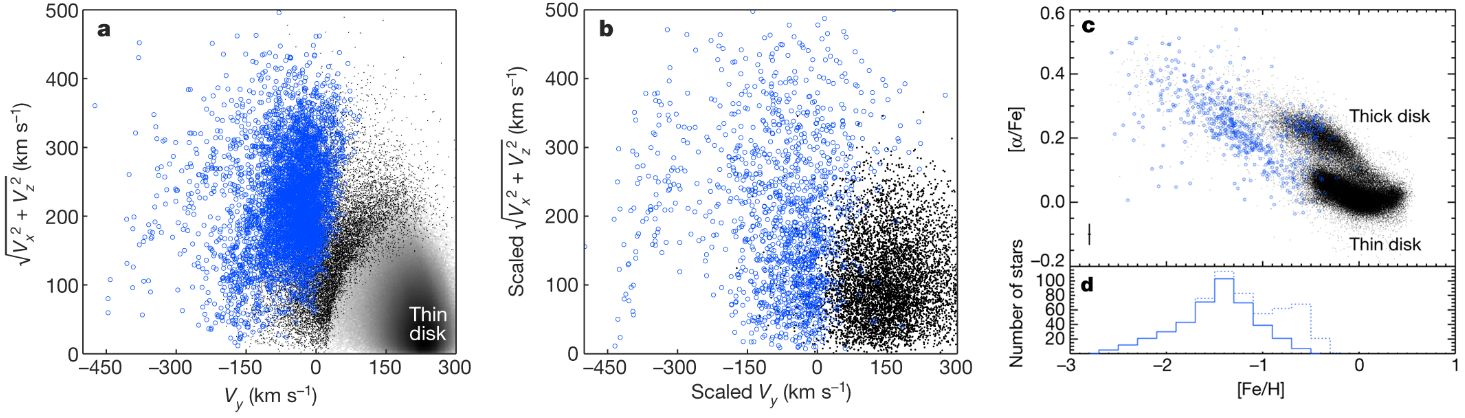
\includegraphics[width=1\textwidth]{./figure/Gaia_Helmi18.png}
    \caption{Left panel: Toomre diagram for Gaia DR2 data where in blue are stars selected to pick out the GSE structure. Middle panel:  similar to the left panel but with simulated data of a minor merger, resulting in a less concentrated structure, mostly due to the fact that a more massive structure is more able to retain its original orbital properties. Right panel: the star in blue are the same of the left panel crossmateched with the APOGEE chemical information.  [The figure is from \cite{helmiMergerThatLed2018}].}
    \label{fig:Gaia_Helmi}
\end{figure}



Robustly identify distinct structure is challenging, and disentangle the components in fully phase mix situations is nearly impossible. In order to characterize the assembly history \cite{cunninghamReadingCARDsImprint2022}
propose to use the "CARDs", the chemical abundance ratio distributions of the stars, obtained from a subsample of accreted object candidate from the FIRE-2 zoom-in cosmological simulations of MW-mass galaxies \cite{wetzelRECONCILINGDWARFGALAXIES2016}. 
Although similar to CASBI on how to leverage $N$-body simulations, this method do not recovers posteriors for the parameters of the accreted objects
but rather considers the host halo as a linear combinations of templates CARDs \begin{equation}
    \text{CARD}_{\text{halo, model}} (x_d) = \sum_i \sum_j A_{ij} \text{CARD}_{\text{temp}, ij} (x_d|M_{\text{sat}, i}, t_{100, j}),
\end{equation} 
treating each coefficient $A_{ij}$ as the fraction of mass contribution from the accretion event of the template satellite with mass $M_{\text{sat}, i}$ and quenching time $t_{100, j}$, and tries to recover those coefficients by maximize a loss that comperes the observed CARDs with the combination of the templates. An example of template constructed from dwarf galaxies is presented in Fig. \ref{fig:CARDS}. The template that were used belong to the catalog of star particles in the FIRE simulations belonging to dwarf galaxies, stellar streams and phase-mixed debris constructed in \cite{panithanpaisalGalaxyProgenitorsStellar2021}. This method and CASBI share two more aspect: 1. Both of these methods are meant to be used on simulations, and the integrations of observational data is not yet implemented, even though theoretically possible. 2. Both rely on the assumption that the chemical space of accreted and isolated dwarf galaxies is very similar, due to ram pressure quenching the star formation history of the accreted object and hence 'freezing' these abundance ratios at the infall time. 

\begin{figure}[h]
    \centering
    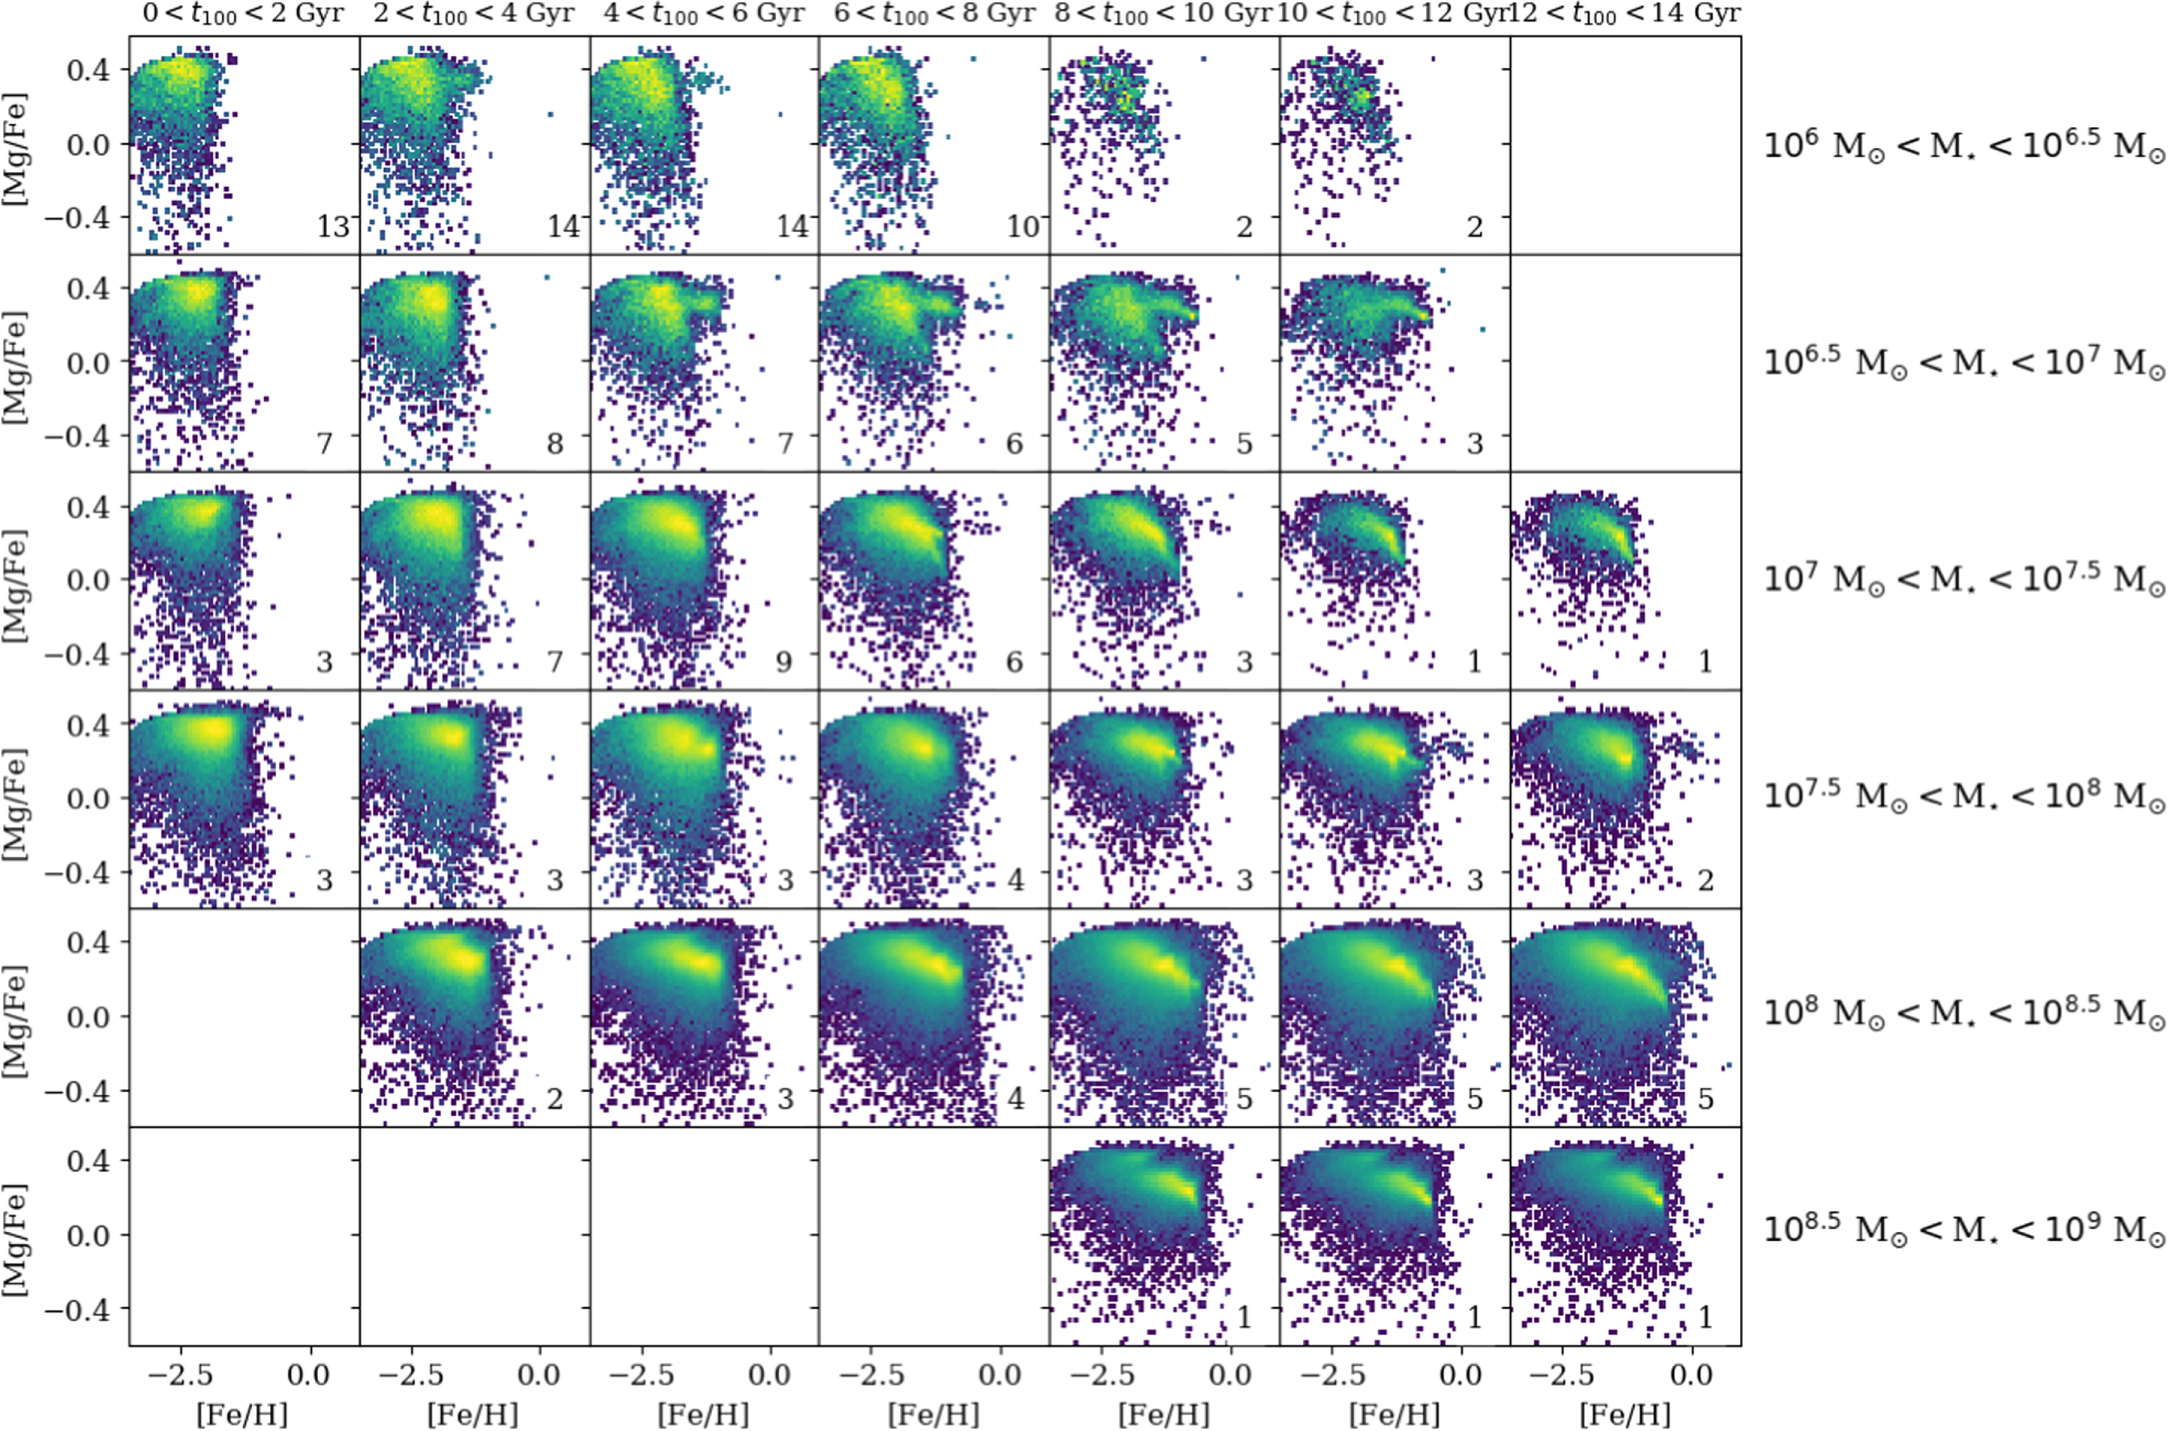
\includegraphics[width=1\textwidth]{./figure/CARDS.jpg}
    \caption{Template for accretion events constructed using dwarf galaxy in \cite{cunninghamReadingCARDsImprint2022}. More massive dwarf galaxies have CARDs that extend to higher metallicities. At fixed stellar mass, galaxies that assemble more quickly (lower $t_{100}$) have more density at higher [Mg/Fe] than the component with a more extended star formation history.}
    \label{fig:CARDS}
\end{figure}

Another approach is presented in \cite{deasonUnravellingMassSpectrum2023}, which takes advantage of the mass-metallicity relation to decompose the metallicity distribution functions (MDF) of the host galaxy as a mixture of accreted halo's MDF, assumed gaussian for each of these building blocks. This assumption are The objective of this work is to obtain a posterior distribution for the number of galaxies in each luminosity bin, which can be considered a proxy for the star mass. In CASBI we adopt the same superimposition philosophy of the components contribution, but we do not assume neither a prefix or an analytical form for the joint distribution of the chemical abundance, relaxing these assumption and relying only on the available samples from the N-body simulations.  